\chapter{Second Approach: Multi-User MISO}

\section{Problem realization}

\subsection{Channel Model}
We assume that our channel model is Rayleigh fading channel model.\\
Consider the centralized massive MISO system, in which the BS is deployed $n_{T_x}$ transmitter antennas and there are $K$ users being randomly distributed in the circular-shape cell. In this scenario, the $n_{T_x}$ transmitter serves to $K$ single-antenna users at the same time frequency resources.\\
Before all users received the transmitted date, the BS shall use some simple linear pre-coding techniques pre-process, which realizes the signal term maximization and interfere term minimization as much as possible. For the $K$ users, the received vector is given by
\[ y = \sqrt{\rho} H W^H s + n \]
where $\rho$ is the input SNR, $\mathbf{H}\in\mathbb{C}^{{K \times n}_{T_x}}$ denotes channel matrix between $n_{T_x}$ transmitter antenna and $K$ users, $\mathbf{s}\in{\mathbb{C}}^{1 \times K}$ denotes a signal vector, $\mathbf{W}\in{\mathbb{C}}^{{K \times n}_{T_x}}$ the pre-coder  matrix, which enables to boosts the total achievable rate of massive multi-user MISO system, $n$ denotes complex-valued additive white Gaussian noise (AWGN) at user, distributed as $\mathcal{N} \mathcal{C} (0, \sigma^\mathbf{2}_\mathbf{n})$.
We assume that the perfect and instantaneous channel state information (CSI) is available at the BS, which can potentially be obtained for massive MISO system, such as in frequency division duplex (FDD) mode, where the BS acquires the perfect CSI through exploiting uplink channel feedback. In time division duplex (TDD) mode, the perfect CSI is acquired by the BS through open-loop uplink pilot training. Before the transmitter symbol, the BS adopts the three different linear pre-coding schemes.\\
At the user's terminal, each user receives a symbol via pre-coding, thus the received signal at the user k is given by:
\begin{equation}
    y_k=h_k\ w_k^H\ s_k+\sum_{j=1,j \neq k}^{K}{h_k\ w_j^H\ s_j}+n_k
\end{equation}
where $h_k \in \mathbb{C}^{1 \times n_{T_x}}$ represents the $k^{th}$ row of the channel matrix $H$, whose entries are i.i.d. complex Gaussian random variable under the Rayleigh fading channel. Similarly, $w_k$ denotes the $k^{th}$ row vector of pre-coding matrix $W$ that satisfies limited condition $s_k$ and $s_j$ represent transmit symbols for the user $k$ and $j$, and $n_k\in \mathcal{N} \mathcal{C}(0,\sigma^\mathbf{2}_n)$.

\subsection{Rate equation}
According to the signal model, we can write the rate equation for the user $k$, which is calculated as
\begin{equation}
    R_k=\log_2\left(1+\frac{{\rho\left|h_k w_k^H\right|}^2}{1+\rho \sum_{j=1,j\neq k}^{K}{\left|h_k w_j^H\right|^2}}\right)
\end{equation}
Where our goal to find the best pre-coding vector $w_k$ which maximizes the overall rate.

\section{Different Pre-coder Constraint Assumption}
\subsection{Model 1 (Power Allocation)}
\subsubsection{Model Constraints}
\begin{itemize}
    \item We impose the power constraint \[\mathbb{E} \left\{ |s_k| \right\} = 1\] where $\mathbb{E}\left\{\cdot\right\}$ denotes the expectation with respect to the distribution of the underlying random variable.
    \item We assume that \[ \sum_{k=1}^{K}\|w_k\|^2_2 = 1\] which means BS sends different power to different users according to its channel coefficient.
\end{itemize}
\subsubsection{Model Optimization Formulation}
As we have mentioned our goal to maximize the sum rate so now we formulate our problem as a standard optimization problem:
\begin{equation}
    \label{eq:multi-user opt pa}
    \begin{aligned}
        \max_{w_k} \quad & \sum_{k=1}^{K} \delta_k  R_k = \sum_{k=1}^{K} \delta_k \log_2 \left( 1 + \frac{\rho | h_k w_k^H |^2}{1 + \rho \sum_{j=1, 1\neq k}^{K}| h_k w_j^H |^2} \right) \\
        \text{s.t.} \quad &  \sum_{k=1}^{K}\|w_k\|^2_2 \leq 1 \\
        & \|s_k\|_2 =1 \quad , \quad k \in [1, \ldots , K] \\
        & \sum_{k=1}^{K} \delta_k = 1 \\
        & h_k, w_k \in \mathbb{C}^{1 \times n_{T_x}}
    \end{aligned}
\end{equation}
since we have constraint on pre-coder where the 2-norm square of pre-coding vector for each user is equal to one, then \[ p_t = \sum_{k=1}^{K}\|w_k s_k\|^2_2 = 1 \] since we have assumed that $\sigma_s =1$
\subsubsection{Achievable Rate for Multi-User MISO System}
We used the known linear pre-coder techniques like MRT (Maximum Ratio Transmission) and ZF (Zero forcing) as the achievable rate analysis for massive MIMO system in this model:
\begin{description}
    \item[Maximum Ratio Transmission (MRT):] \[ w_{\text{MRT}} = \frac{H}{\sqrt{\|h_1\|_2^2 + \ldots + \|h_k\|_2^2}} \]
    \item[Zero Forcing (ZF):] Let $G = \left( H H^H \right)^{-1} H$ \[ w_{\text{ZF}} = \frac{G}{\sqrt{\|g_1\|_2^2 + \ldots + \|g_k\|_2^2}} \]where $H, G, w \in \mathbb{C}^{K \times n_{T_x}}$ and $h_k, g_k \in \mathbb{C}^{1 \times n_{T_x}}$.
\end{description}
So, $w_{\text{MRT}}$ and $w_{\text{ZF}}$ achieve the constraint $\sum_{k=1}^{K}\|w_k\|^2_2 = 1$.

\subsection{Model 2 (Equally Transmitted Power to All Users)}
\subsubsection{Model Constraints}
\begin{itemize}
    \item We impose the power constraint \[\mathbb{E} \left\{ |s_k| \right\} = 1\] where $\mathbb{E}\left\{\cdot\right\}$ denotes the expectation with respect to the distribution of the underlying random variable.
    \item We assume that \[ \|w_k\|_2 = 1\] which means each user takes the same power from BS.
\end{itemize}
\subsubsection{Model Optimization Formulation}
As we have mentioned our goal to maximize the sum rate so now we formulate our problem as a standard optimization problem:
\begin{equation}
    \label{eq:multi-user opt sp}
    \begin{aligned}
        \max_{w_k} \quad & \sum_{k=1}^{K} \delta_k R_k = \sum_{k=1}^{K} \delta_k \log_2 \left( 1 + \frac{\rho | h_k w_k^H |^2}{1 + \rho \sum_{j=1, 1\neq k}^{K}| h_k w_j^H |^2} \right) \\
        \text{s.t.} \quad &  \|w_k\|_2 = 1 \\
        & \|s_k\|_2 =1 \quad , \quad k \in [1, \ldots , K] \\
        & \sum_{k=1}^{K} \delta_k = 1 \\
        & h_k, w_k \in \mathbb{C}^{1 \times n_{T_x}}
    \end{aligned}
\end{equation}
since we have constraint on pre-coding where the 2-norm square of pre-coding vector for each user is equal to one, then
\[ p_t = \sum_{k=1}^{K}\|w_k s_k\|^2_2 = 4 \]
since we have assumed that $\sigma_s =1$
\subsubsection{Achievable Rate for Multi-User MISO System}
We used the known linear pre-coder techniques like MRT (Maximum Ratio Transmission) and ZF (Zero forcing) as the achievable rate analysis for massive MIMO system in this model:
\begin{description}
    \item[Maximum Ratio Transmission (MRT):] \[ w_k^{\text{MRT}} = \frac{h_k}{\|h_k\|_2} \quad , \quad k \in [1, \ldots , K] \]
    \item[Zero Forcing (ZF):] Let $G = \left( H H^H \right)^{-1} H$ \[ w_k^{\text{ZF}} = \frac{g_k}{\|g_k\|_2} \quad , \quad k \in [1, \ldots , K] \]where $H, G, w \in \mathbb{C}^{K \times n_{T_x}}$ and $h_k, g_k \in \mathbb{C}^{1 \times n_{T_x}}$.
\end{description}
So, $w_{\text{MRT}}$ and $w_{\text{ZF}}$ achieve the constraint $\|w_k\|_2 = 1$.

\section{RL Interpretation}
\subsection{Introduction}
The problem of assignment precoder for multi user to maximize the rate with low interference doesn't have the optimal solution, so we use DRL techniques especially DDPG to try to find the best solution for this problem because RL uses the reward to search about the action which give the high cumulative reward.
\subsection{Problem Mapping}
Now let's define the state, action and reward to map our optimization problem to RL.
\begin{description}
    \item[State:] $S_t=H_t$, but $H_t$ is a complex matrix which has a size $({K \times n}_{T_x})$, and as we have mentioned that neural networks don't take a complex as input so we define the state \[ S_t = \left[ \Re(H_t) , \Im(H_t) \right] \]So $S_t \in \mathbb{R}^{k \times 2n_{T_x}}$
    \item[Action:] $A_t = actor_{\theta^a} (S_t)$ where $A_t \in \mathbb{R}^{k \times 2n_{T_x}}$ but the pre-coder must be a complex so we will turn $A_t$ to complex by split $A_t$ to two halves by columns \[ W_t = A_{1:n_{T_x}} + \jmath A_{n_{T_x}+1 : 2n_{T_x}} \]where $A_{1:n_{T_x}}$ has a size of $(k \times n_{T_x})$
    \item[Reward:] Sum average reward, where $R_k$ is the rate us the user.\[r_t = \sum_{k=1}^{K} \delta_k R_k \quad , \quad K, r_t \in \mathbb{R}\]
\end{description}
\subsection{Algorithm Parameters}
\begin{enumerate}
    \item 3 hidden layers model with neurons [1024,512,128] respectively.
    \item Actor learning rate = 0.001 and Critic learning rate = 0.002 with decaying reaches to 0.0001 and 0.0002 respectively.
    \item Channel noise = 0.2 in case of low input SNR.
    \item Exploration noise variance \[ \sigma^2_\epsilon = \frac{0.1}{\text{episode number}} \]
    \item $\alpha, \beta, \gamma \in [0,1]$
\end{enumerate}

\section{Evaluation}
\subsection{In Low SNR}
\subsubsection{Model 1 (Power Allocation)}
\begin{figure}[H]
    \centering
    \begin{subfigure}{.5\textwidth}
      \centering
      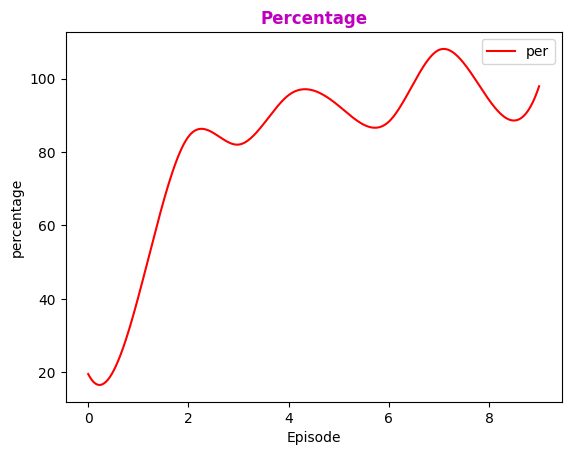
\includegraphics[width=.85\linewidth]{Ha1.png}
      \caption{Actor's to MRT's average reward}
      \label{fig:lowSNR Model1}
    \end{subfigure}%
    \begin{subfigure}{.5\textwidth}
      \centering
      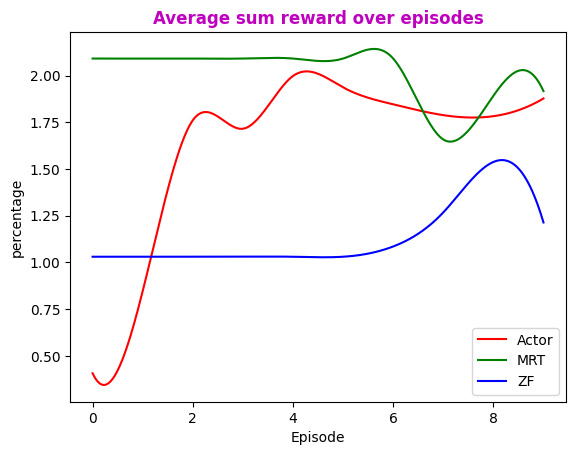
\includegraphics[width=.85\linewidth]{Ha2.png}
      \caption{Average reward}
      \label{fig:lowSNR Model1_1}
    \end{subfigure}
\end{figure}
\textbf{On average:}
\begin{itemize}
    \item Percentage subject to MRT= 100.43\%
    \item Percentage subject to ZF= 157.84\%
\end{itemize}
The MRT has the performance better than ZF in low SNR, we will check our model using MRT, we observe that our model exceeds the MRT performance and it have not reached to convergence yet.
\subsubsection{Model 2 (Fairness)}
\textbf{On average: (after $30 \times {10}^4$ iterations)}
    \begin{itemize}
        \item Percentage subject to MRT= 96.71\%
        \item Percentage subject to ZF= 129.8\%
    \end{itemize}

\subsection{In High SNR}
\subsubsection{Model 1 (Power Allocation)}
We have 2 versions of the model:
\begin{enumerate}
    \item \textbf{Log reward:}
    \begin{equation}
        \label{eq:Log reward model 1}
        r_t=\sum_{k=1}^{K}{\delta_k \log_2 \left(1+\frac{{{\rho}\left|{h}_{k}\ {w}_{k}^{H}\right|}2}{{1}+{\rho}\ \sum_{{j}={1},{j}\neq{k}}^{{K}}{\left|{h}_{k}\ {w}_{j}^{H}\right|^{2}\ }}\right)}
    \end{equation}
    \begin{figure}[H]
        \centering
        \begin{subfigure}{.5\textwidth}
          \centering
          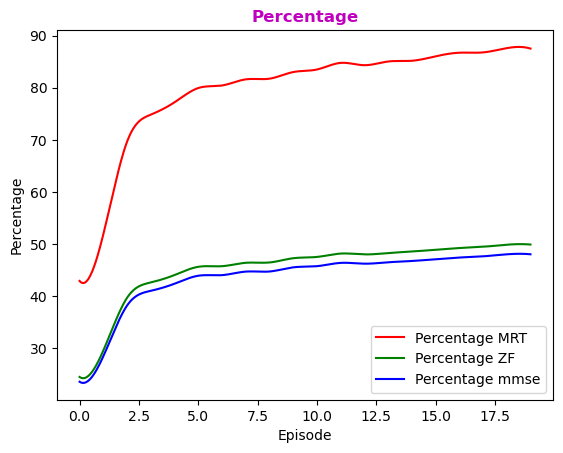
\includegraphics[width=.85\linewidth]{Ha3.png}
          \caption{\% of actor reward to MRT's \& ZF's \& MMSE's}
          \label{fig:highSNR Model1}
        \end{subfigure}%
        \begin{subfigure}{.5\textwidth}
          \centering
          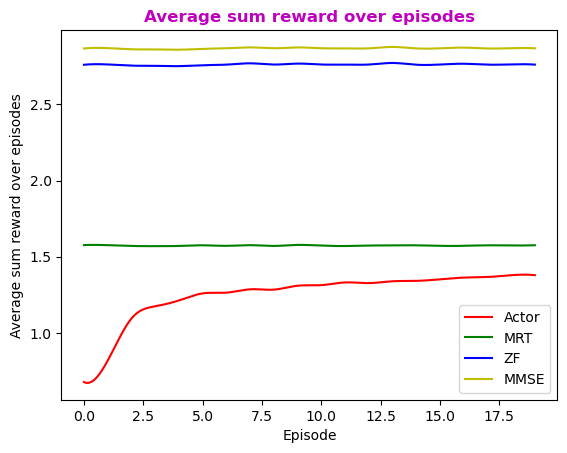
\includegraphics[width=.85\linewidth]{Ha4.png}
          \caption{Average reward}
          \label{fig:highSNR Model1_1}
        \end{subfigure}
    \end{figure}
    \textbf{On average: (after $20 \times {10}^4$ iterations)}
    \begin{itemize}
        \item Percentage subject to MRT= 87.3\%
        \item Percentage subject to ZF= 49.76\%
        \item Percentage subject to MMSE= 47.93\%
    \end{itemize}
    Since we have not resource and the model is extremely complex, the model needs at least 400 episodes to converge but we train it 30 episodes only, so it will reach to MMSE and can pass it, but it needs more computational power.\\
    \textbf{Reshaped reward:}
    \begin{equation}
        \label{eq:reshaped model}
        \begin{aligned}
            {r}_{t} & = \sum_{{k}=1}^{{K}}{{{\delta}_{k} \log}_{2}\ \left(1+\frac{{{\rho}\left|{h}_{k}\ {w}_{k}^{H}\right|}^{2}}{{1}+{\rho}\ \sum_{{j}={1},{j}\neq{k}}^{{K}}{\left|{h}_{k}\ {w}_{j}^{H}\right|^{2}\ }}\right)} \\
            & - \sum_{{k}={1}}^{{K}}{{\delta}_{k} \log_2\ \left({1}+\frac{{{\rho}\left|{h}_{k}\ {{w}_{k}^{{\text{MMSE}}}}^{H}\right|}^{2}}{{1}+{\rho}\ \sum_{{j}={1},{j}\neq{k}}^{{K}}{\left|{h}_{k}\ {{w}_{j}^{{\text{MMSE}}}}^{H}\right|^{2}\ }}\right)}\\
            & + {0}.{5}
        \end{aligned}
    \end{equation}
    \begin{figure}[H]
        \centering
        \begin{subfigure}{.5\textwidth}
          \centering
          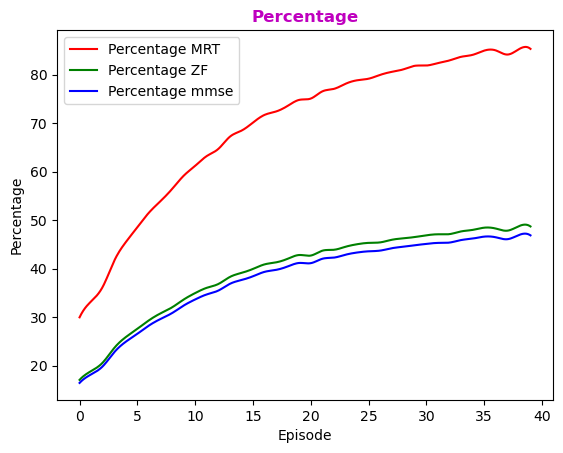
\includegraphics[width=.85\linewidth]{Ha5.png}
          \caption{\% of actor reward to MRT's \& ZF's \& MMSE's}
          \label{fig:highSNR Model1-reshaped}
        \end{subfigure}%
        \begin{subfigure}{.5\textwidth}
          \centering
          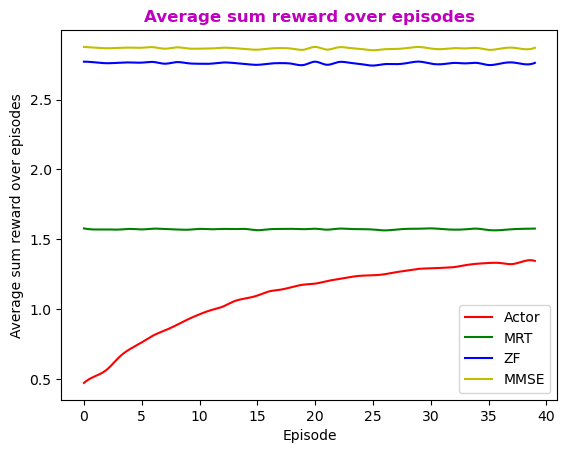
\includegraphics[width=.85\linewidth]{Ha6.png}
          \caption{Average reward}
          \label{fig:highSNR Model1_1-reshaped}
        \end{subfigure}
    \end{figure}
    \textbf{On average: (after $26 \times {10}^4$ iterations)}
    \begin{itemize}
        \item Percentage subject to MRT= 85.11\%
        \item Percentage subject to ZF= 48.6\%
        \item Percentage subject to MMSE= 46.76\%
    \end{itemize}
\end{enumerate}

\subsubsection{Model 2 (Fairness)}
\textbf{On average: (after $26 \times {10}^4$ iterations)}
\begin{itemize}
    \item Percentage subject to MRT= 95.9\%
    \item Percentage subject to ZF= 34.77\%
    \item Percentage subject to MMSE= 34.33\%
\end{itemize}
\begin{figure}[H]
    \centering
    \begin{subfigure}{.5\textwidth}
      \centering
      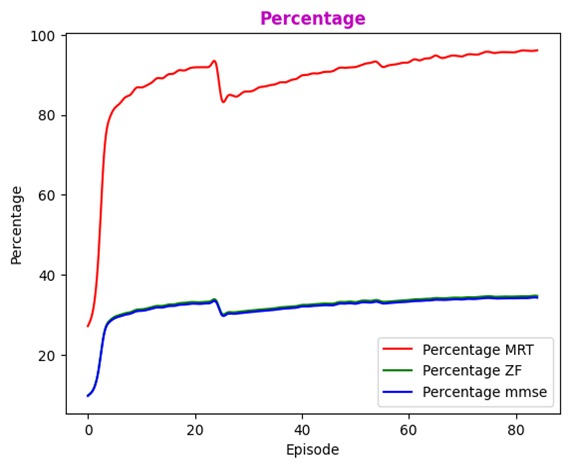
\includegraphics[width=.85\linewidth]{Ha11.jpg}
      \caption{\% of actor reward to MRT's \& ZF's \& MMSE's}
      \label{fig:highSNR Model1-reshaped}
    \end{subfigure}%
    \begin{subfigure}{.5\textwidth}
      \centering
      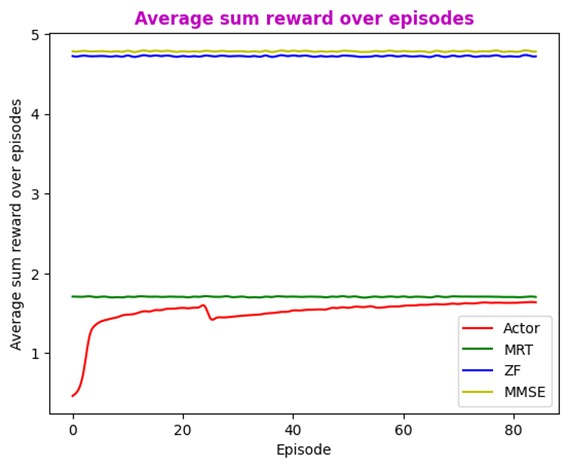
\includegraphics[width=.85\linewidth]{Ha12.jpg}
      \caption{Average reward}
      \label{fig:highSNR Model1_1-reshaped}
    \end{subfigure}
\end{figure}

\section{Architecture of Other Trials}
\subsection{Batch Normalize Layers}
Batch normalization is a technique for training very deep neural networks that standardizes the inputs to a layer for each mini-batch. This has the effect of stabilizing the learning process and dramatically reducing the number of training epochs required to train deep networks by avoiding vanishing and exploding of gradient. \\
There are 2 versions of this model depending on the activation function:
\begin{description}
    \item[Relu activation function:] Here we used 'relu' activation function with batch normalize, the performance of in case of model 1 and high SNR is 
    \begin{figure}[H]
        \centering
        \begin{subfigure}{.5\textwidth}
          \centering
          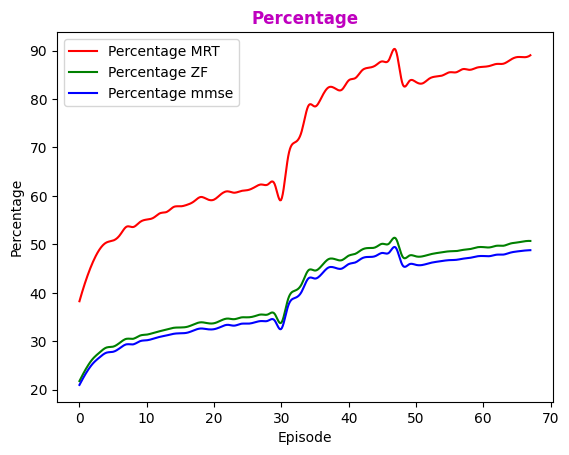
\includegraphics[width=.85\linewidth]{Ha7.png}
          \caption{\% of actor reward to MRT's \& ZF's \& MMSE's}
          \label{fig:btl}
        \end{subfigure}%
        \begin{subfigure}{.5\textwidth}
          \centering
          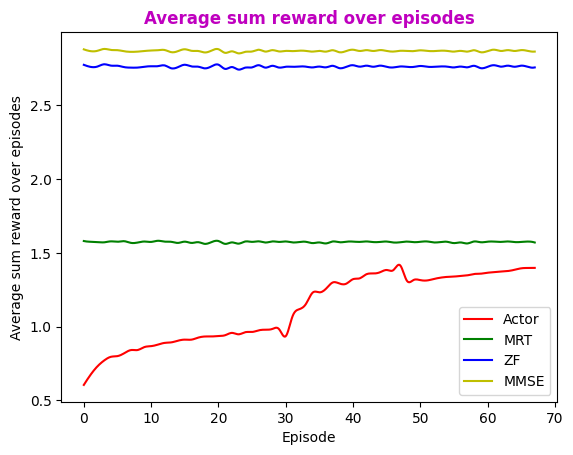
\includegraphics[width=.85\linewidth]{Ha8.png}
          \caption{Average reward}
          \label{fig:btl-1}
        \end{subfigure}
    \end{figure}
    \textbf{On average: (after 70 concatenated episodes)}
    \begin{itemize}
        \item Percentage subject to MRT= 88.55\% 
        \item Percentage subject to ZF= 50.58\% 
        \item Percentage subject to MMSE= 48.69\%
    \end{itemize}
    \item[Tanh activation function:] Here we used 'tanh' activation function with batch normalize, the performance of in case of model 1 and high SNR is 
    \begin{figure}[H]
        \centering
        \begin{subfigure}{.5\textwidth}
          \centering
          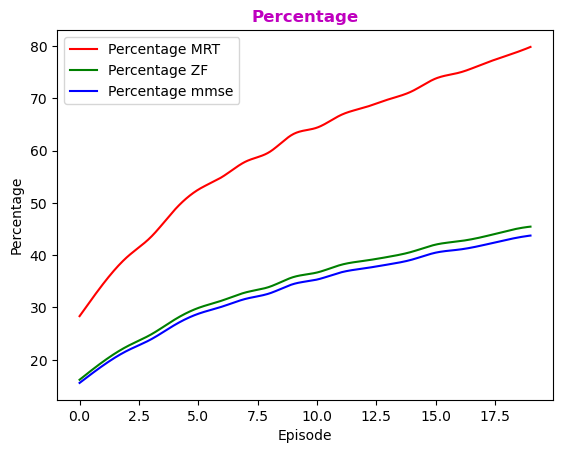
\includegraphics[width=.85\linewidth]{Ha9.png}
          \caption{\% of actor reward to MRT's \& ZF's \& MMSE's}
          \label{fig:tanh}
        \end{subfigure}%
        \begin{subfigure}{.5\textwidth}
          \centering
          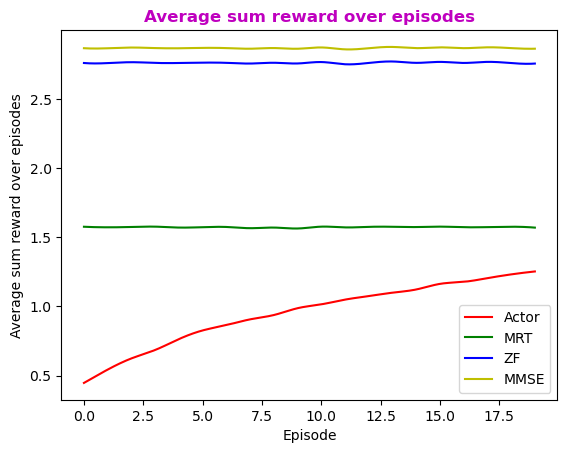
\includegraphics[width=.85\linewidth]{Ha10.png}
          \caption{Average reward}
          \label{fig:tanh-1}
        \end{subfigure}
    \end{figure}
    \textbf{On average: (after 20 episodes)}
    \begin{itemize}
        \item Percentage subject to MRT= 79.49\% 
        \item Percentage subject to ZF= 45.41\% 
        \item Percentage subject to MMSE= 43.71\%
    \end{itemize}
\end{description}
\subsection{Skip Connection}
Skip Connections were introduced to solve different problems in different architectures. In the case of ResNets, skip connections solved the degradation problem that we addressed earlier whereas, in the case of DenseNets, it ensured feature reusability. \\
We try to use it here to add regularization and decrease the complexity of the critic network.

\section{Future Work}
\subsection{General Model}
High and low SNR at same time, input SNR chosen randomly between $[-10dB,\ 10dB]$.\\
The difference here is in the state, here state is the channel coefficient matrix ($H_t$) in addition to input SNR ($\rho$).
\subsection{Connect ML with RL}
The MMSE pre-coder technique achieves the rate greater than MRT an ZF, so we will try to train an ordinary neural network that labeled by the pre-coder of MMSE so after training the NN will act like MMSE then we will transfer its weights to the actor network and then start soft update using RL to try to achieve better performance.
